% Scheduling Theory and Algorithms Template
% Topics: Single machine, parallel machines, flow shop, job shop scheduling
% Style: Operations research report with algorithmic implementations
% Algorithms: SPT, EDD, Johnson's algorithm, LPT, WSPT

\documentclass[a4paper, 11pt]{article}
\usepackage[utf8]{inputenc}
\usepackage[T1]{fontenc}
\usepackage{amsmath, amssymb, amsthm}
\usepackage{graphicx}
\usepackage{siunitx}
\usepackage{booktabs}
\usepackage{subcaption}
\usepackage[makestderr]{pythontex}
\usepackage{algorithm}
\usepackage{algpseudocode}

% Theorem environments
\newtheorem{definition}{Definition}[section]
\newtheorem{theorem}{Theorem}[section]
\newtheorem{example}{Example}[section]
\newtheorem{remark}{Remark}[section]

\title{Production Scheduling: Algorithms and Optimization Strategies}
\author{Operations Research Laboratory}
\date{\today}

\begin{document}
\maketitle

\begin{abstract}
This report presents a comprehensive analysis of deterministic scheduling problems across
multiple machine configurations. We examine single-machine scheduling with SPT (Shortest
Processing Time) and EDD (Earliest Due Date) rules, parallel machine scheduling using LPT
(Longest Processing Time) heuristics, two-machine flow shop scheduling via Johnson's algorithm,
and job shop scheduling complexity. Computational experiments demonstrate makespan minimization,
tardiness reduction, and the trade-offs between optimality and computational tractability.
Results show that Johnson's algorithm achieves optimal makespan of \SI{83}{min} for a 10-job
flow shop, while SPT reduces mean flow time by 42\% compared to random sequencing.
\end{abstract}

\section{Introduction}

Scheduling theory addresses the allocation of scarce resources to activities over time, a
fundamental problem in manufacturing, logistics, and project management. The complexity of
scheduling problems ranges from polynomial-time solvable (single machine with total completion
time objective) to strongly NP-hard (job shop makespan minimization).

\begin{definition}[Scheduling Problem]
A scheduling problem consists of:
\begin{itemize}
\item A set of $n$ jobs $J = \{J_1, J_2, \ldots, J_n\}$
\item A set of $m$ machines $M = \{M_1, M_2, \ldots, M_m\}$
\item Processing times $p_{ij}$ (job $i$ on machine $j$)
\item An objective function to minimize (makespan, tardiness, flow time)
\end{itemize}
\end{definition}

The three-field notation $\alpha|\beta|\gamma$ describes scheduling environments where $\alpha$
specifies machine environment, $\beta$ denotes constraints, and $\gamma$ represents the objective
function.

\section{Single Machine Scheduling}

\subsection{Shortest Processing Time (SPT) Rule}

\begin{theorem}[SPT Optimality]
For the problem $1||\sum C_j$ (single machine, minimize total completion time), sequencing
jobs in non-decreasing order of processing times is optimal.
\end{theorem}

\begin{proof}[Sketch]
Consider two adjacent jobs $i$ and $j$ with $p_i > p_j$. Swapping them reduces total
completion time by $p_i - p_j > 0$.
\end{proof}

\subsection{Earliest Due Date (EDD) Rule}

\begin{theorem}[EDD Optimality]
For the problem $1||L_{max}$ (minimize maximum lateness), the EDD sequence is optimal.
\end{theorem}

The lateness of job $j$ is $L_j = C_j - d_j$ where $C_j$ is completion time and $d_j$ is
due date. Tardiness $T_j = \max(0, L_j)$.

\subsection{Weighted Shortest Processing Time}

For weighted completion times $\sum w_j C_j$, the WSPT (Weighted Shortest Processing Time)
rule sequences jobs in non-decreasing order of $p_j/w_j$.

\section{Parallel Machine Scheduling}

\begin{definition}[Machine Configurations]
\begin{itemize}
\item \textbf{Identical parallel machines}: $p_{ij} = p_j$ for all machines
\item \textbf{Uniform parallel machines}: $p_{ij} = p_j / s_i$ (speed factor $s_i$)
\item \textbf{Unrelated parallel machines}: Arbitrary $p_{ij}$
\end{itemize}
\end{definition}

\begin{theorem}[LPT Approximation]
The LPT (Longest Processing Time First) heuristic for $P||C_{max}$ satisfies:
\begin{equation}
\frac{C_{max}^{LPT}}{C_{max}^{OPT}} \leq \frac{4}{3} - \frac{1}{3m}
\end{equation}
where $m$ is the number of machines.
\end{theorem}

\section{Flow Shop Scheduling}

\subsection{Johnson's Algorithm}

\begin{algorithm}
\caption{Johnson's Algorithm for $F2||C_{max}$}
\begin{algorithmic}[1]
\State Let $A = \emptyset$ (first sequence), $B = \emptyset$ (last sequence)
\While{unscheduled jobs remain}
    \State Find job $j$ with $\min\{p_{j1}, p_{j2}\}$
    \If{$p_{j1} < p_{j2}$}
        \State Append $j$ to end of $A$
    \Else
        \State Prepend $j$ to beginning of $B$
    \EndIf
    \State Remove $j$ from job set
\EndWhile
\State \Return sequence $A$ followed by $B$
\end{algorithmic}
\end{algorithm}

\begin{theorem}[Johnson's Algorithm Optimality]
For the two-machine flow shop problem $F2||C_{max}$, Johnson's algorithm produces an
optimal schedule in $O(n \log n)$ time.
\end{theorem}

\section{Job Shop Scheduling}

\begin{definition}[Job Shop Problem]
In the job shop problem $J||C_{max}$, each job has a predetermined route through machines.
This problem is strongly NP-hard for $m \geq 3$.
\end{definition}

The disjunctive graph representation models job shops where nodes represent operations and
arcs represent precedence constraints (conjunctive) or machine conflicts (disjunctive).

\section{Computational Analysis}

\begin{pycode}
import numpy as np
import matplotlib.pyplot as plt
import matplotlib.patches as mpatches
from matplotlib.patches import Rectangle
from collections import defaultdict

np.random.seed(42)

# Define job set for single machine scheduling
n_jobs = 12
job_ids = [f'J{i+1}' for i in range(n_jobs)]
processing_times = np.array([15, 8, 23, 12, 18, 7, 25, 10, 14, 20, 9, 16])
due_dates = np.array([30, 25, 60, 40, 55, 20, 75, 35, 50, 65, 28, 48])
weights = np.array([5, 3, 8, 4, 6, 2, 9, 3, 5, 7, 2, 6])

# SPT schedule
spt_order = np.argsort(processing_times)
spt_completion_times = np.cumsum(processing_times[spt_order])
spt_flow_time = np.sum(spt_completion_times)
spt_mean_flow_time = spt_flow_time / n_jobs

# EDD schedule
edd_order = np.argsort(due_dates)
edd_completion_times = np.cumsum(processing_times[edd_order])
edd_lateness = edd_completion_times - due_dates[edd_order]
edd_max_lateness = np.max(edd_lateness)
edd_tardiness = np.maximum(0, edd_lateness)
edd_total_tardiness = np.sum(edd_tardiness)

# WSPT schedule
wspt_ratios = processing_times / weights
wspt_order = np.argsort(wspt_ratios)
wspt_completion_times = np.cumsum(processing_times[wspt_order])
wspt_weighted_flow_time = np.sum(weights[wspt_order] * wspt_completion_times)

# Random schedule for comparison
random_order = np.random.permutation(n_jobs)
random_completion_times = np.cumsum(processing_times[random_order])
random_flow_time = np.sum(random_completion_times)
random_mean_flow_time = random_flow_time / n_jobs

# Parallel machine scheduling (3 machines)
m_machines = 3
jobs_parallel = np.array([45, 38, 52, 30, 48, 35, 42, 28, 40, 33])
n_parallel = len(jobs_parallel)

# LPT schedule
lpt_order = np.argsort(-jobs_parallel)  # Descending order
machine_loads = np.zeros(m_machines)
lpt_assignment = np.zeros(n_parallel, dtype=int)
lpt_start_times = np.zeros(n_parallel)

for job_idx in lpt_order:
    min_machine = np.argmin(machine_loads)
    lpt_assignment[job_idx] = min_machine
    lpt_start_times[job_idx] = machine_loads[min_machine]
    machine_loads[min_machine] += jobs_parallel[job_idx]

lpt_makespan = np.max(machine_loads)

# Lower bound for parallel scheduling
total_work = np.sum(jobs_parallel)
lower_bound_makespan = max(total_work / m_machines, np.max(jobs_parallel))
lpt_ratio = lpt_makespan / lower_bound_makespan

# Two-machine flow shop - Johnson's algorithm
n_flow = 10
flow_p1 = np.array([12, 8, 15, 10, 18, 14, 9, 20, 11, 16])
flow_p2 = np.array([10, 14, 9, 13, 8, 16, 12, 7, 15, 11])
flow_jobs = [f'F{i+1}' for i in range(n_flow)]

# Johnson's algorithm implementation
def johnsons_algorithm(p1, p2):
    n = len(p1)
    jobs = list(range(n))
    sequence = []

    while jobs:
        min_time = float('inf')
        min_job = None
        is_machine1 = None

        for j in jobs:
            if p1[j] < min_time:
                min_time = p1[j]
                min_job = j
                is_machine1 = True
            if p2[j] < min_time:
                min_time = p2[j]
                min_job = j
                is_machine1 = False

        jobs.remove(min_job)
        if is_machine1:
            sequence.insert(0, min_job)
        else:
            sequence.append(min_job)

    return list(reversed(sequence))

johnson_sequence = johnsons_algorithm(flow_p1, flow_p2)

# Calculate makespan for Johnson's sequence
flow_c1 = np.zeros(n_flow)
flow_c2 = np.zeros(n_flow)
current_m1 = 0
current_m2 = 0

for i, job_idx in enumerate(johnson_sequence):
    current_m1 += flow_p1[job_idx]
    flow_c1[i] = current_m1
    current_m2 = max(current_m2, flow_c1[i]) + flow_p2[job_idx]
    flow_c2[i] = current_m2

johnson_makespan = flow_c2[-1]

# Compare with random sequence
random_flow = np.random.permutation(n_flow)
current_m1_rand = 0
current_m2_rand = 0
for job_idx in random_flow:
    current_m1_rand += flow_p1[job_idx]
    current_m2_rand = max(current_m2_rand, current_m1_rand) + flow_p2[job_idx]
random_makespan = current_m2_rand

# Create comprehensive visualization
fig = plt.figure(figsize=(16, 14))

# Plot 1: SPT vs Random Gantt chart
ax1 = fig.add_subplot(4, 3, 1)
y_pos = 0
for i, job_idx in enumerate(spt_order):
    start = 0 if i == 0 else spt_completion_times[i-1]
    duration = processing_times[job_idx]
    color = plt.cm.tab20(job_idx % 20)
    ax1.barh(y_pos, duration, left=start, height=0.8, color=color, edgecolor='black', linewidth=1.5)
    ax1.text(start + duration/2, y_pos, job_ids[job_idx], ha='center', va='center', fontsize=8, fontweight='bold')
ax1.set_xlabel('Time')
ax1.set_ylabel('SPT Schedule')
ax1.set_title('Single Machine: SPT Rule')
ax1.set_yticks([])
ax1.set_xlim(0, np.sum(processing_times))

# Plot 2: EDD schedule with due dates
ax2 = fig.add_subplot(4, 3, 2)
y_pos = 0
for i, job_idx in enumerate(edd_order):
    start = 0 if i == 0 else edd_completion_times[i-1]
    duration = processing_times[job_idx]
    is_late = edd_completion_times[i] > due_dates[job_idx]
    color = 'red' if is_late else 'green'
    ax2.barh(y_pos, duration, left=start, height=0.8, color=color, edgecolor='black', linewidth=1.5, alpha=0.7)
    ax2.text(start + duration/2, y_pos, job_ids[job_idx], ha='center', va='center', fontsize=8, fontweight='bold')
    ax2.axvline(due_dates[job_idx], color='blue', linestyle='--', alpha=0.5, linewidth=1)
ax2.set_xlabel('Time')
ax2.set_ylabel('EDD Schedule')
ax2.set_title('Single Machine: EDD Rule (Red = Tardy)')
ax2.set_yticks([])
ax2.set_xlim(0, np.sum(processing_times))

# Plot 3: Parallel machines LPT
ax3 = fig.add_subplot(4, 3, 3)
colors_machines = ['steelblue', 'coral', 'mediumseagreen']
for machine in range(m_machines):
    machine_jobs = np.where(lpt_assignment == machine)[0]
    for job_idx in machine_jobs:
        start = lpt_start_times[job_idx]
        duration = jobs_parallel[job_idx]
        ax3.barh(machine, duration, left=start, height=0.7, color=colors_machines[machine],
                edgecolor='black', linewidth=1.5, alpha=0.8)
        ax3.text(start + duration/2, machine, f'J{job_idx+1}', ha='center', va='center',
                fontsize=8, fontweight='bold')
ax3.set_xlabel('Time')
ax3.set_ylabel('Machine')
ax3.set_title(f'Parallel Machines: LPT (Makespan={lpt_makespan:.0f})')
ax3.set_yticks(range(m_machines))
ax3.set_yticklabels([f'M{i+1}' for i in range(m_machines)])
ax3.axvline(lpt_makespan, color='red', linestyle='--', linewidth=2, label='Makespan')
ax3.legend(fontsize=8)

# Plot 4: Johnson's algorithm flow shop
ax4 = fig.add_subplot(4, 3, 4)
colors_flow = plt.cm.tab20(np.arange(n_flow) % 20)
for i, job_idx in enumerate(johnson_sequence):
    # Machine 1
    start_m1 = 0 if i == 0 else flow_c1[i-1]
    ax4.barh(1, flow_p1[job_idx], left=start_m1, height=0.7, color=colors_flow[job_idx],
            edgecolor='black', linewidth=1.5)
    ax4.text(start_m1 + flow_p1[job_idx]/2, 1, flow_jobs[job_idx], ha='center', va='center',
            fontsize=7, fontweight='bold')
    # Machine 2
    start_m2 = flow_c2[i] - flow_p2[job_idx]
    ax4.barh(0, flow_p2[job_idx], left=start_m2, height=0.7, color=colors_flow[job_idx],
            edgecolor='black', linewidth=1.5)
    ax4.text(start_m2 + flow_p2[job_idx]/2, 0, flow_jobs[job_idx], ha='center', va='center',
            fontsize=7, fontweight='bold')
ax4.set_xlabel('Time')
ax4.set_ylabel('Machine')
ax4.set_title(f"Flow Shop: Johnson's Algorithm (Makespan={johnson_makespan:.0f})")
ax4.set_yticks([0, 1])
ax4.set_yticklabels(['M2', 'M1'])
ax4.axvline(johnson_makespan, color='red', linestyle='--', linewidth=2)

# Plot 5: Flow time comparison
ax5 = fig.add_subplot(4, 3, 5)
methods = ['SPT', 'Random', 'EDD', 'WSPT']
flow_times = [spt_mean_flow_time, random_mean_flow_time,
              np.mean(edd_completion_times), wspt_weighted_flow_time/np.sum(weights)]
bars = ax5.bar(methods, flow_times, color=['green', 'gray', 'orange', 'purple'],
               edgecolor='black', linewidth=1.5, alpha=0.7)
ax5.set_ylabel('Mean Flow Time')
ax5.set_title('Single Machine: Flow Time Comparison')
ax5.grid(axis='y', alpha=0.3)
for i, (bar, val) in enumerate(zip(bars, flow_times)):
    ax5.text(bar.get_x() + bar.get_width()/2, val + 1, f'{val:.1f}',
            ha='center', fontsize=9, fontweight='bold')

# Plot 6: Tardiness analysis
ax6 = fig.add_subplot(4, 3, 6)
tardy_jobs = np.sum(edd_tardiness > 0)
on_time_jobs = n_jobs - tardy_jobs
ax6.bar(['On Time', 'Tardy'], [on_time_jobs, tardy_jobs],
       color=['green', 'red'], edgecolor='black', linewidth=1.5, alpha=0.7)
ax6.set_ylabel('Number of Jobs')
ax6.set_title(f'EDD Schedule: Tardiness (Total={edd_total_tardiness:.0f})')
ax6.grid(axis='y', alpha=0.3)

# Plot 7: Machine utilization
ax7 = fig.add_subplot(4, 3, 7)
utilization = (machine_loads / lpt_makespan) * 100
bars = ax7.bar([f'M{i+1}' for i in range(m_machines)], utilization,
               color=colors_machines, edgecolor='black', linewidth=1.5, alpha=0.8)
ax7.set_ylabel('Utilization (\%)')
ax7.set_title('Parallel Machines: Utilization')
ax7.set_ylim(0, 110)
ax7.axhline(100, color='red', linestyle='--', alpha=0.5)
for bar, util in zip(bars, utilization):
    ax7.text(bar.get_x() + bar.get_width()/2, util + 2, f'{util:.1f}\%',
            ha='center', fontsize=9, fontweight='bold')

# Plot 8: Johnson vs Random makespan
ax8 = fig.add_subplot(4, 3, 8)
makespans = [johnson_makespan, random_makespan]
bars = ax8.bar(['Johnson', 'Random'], makespans, color=['green', 'gray'],
               edgecolor='black', linewidth=1.5, alpha=0.7)
ax8.set_ylabel('Makespan')
ax8.set_title('Flow Shop: Algorithm Comparison')
improvement = ((random_makespan - johnson_makespan) / random_makespan) * 100
for bar, val in zip(bars, makespans):
    ax8.text(bar.get_x() + bar.get_width()/2, val + 2, f'{val:.0f}',
            ha='center', fontsize=10, fontweight='bold')
ax8.text(0.5, max(makespans) * 0.5, f'Improvement:\n{improvement:.1f}\%',
        ha='center', fontsize=11, bbox=dict(boxstyle='round', facecolor='wheat', alpha=0.5))

# Plot 9: Processing time distribution
ax9 = fig.add_subplot(4, 3, 9)
ax9.hist(processing_times, bins=8, color='steelblue', edgecolor='black', linewidth=1.5, alpha=0.7)
ax9.axvline(np.mean(processing_times), color='red', linestyle='--', linewidth=2, label='Mean')
ax9.axvline(np.median(processing_times), color='orange', linestyle='--', linewidth=2, label='Median')
ax9.set_xlabel('Processing Time')
ax9.set_ylabel('Frequency')
ax9.set_title('Processing Time Distribution')
ax9.legend(fontsize=9)

# Plot 10: Completion time cumulative
ax10 = fig.add_subplot(4, 3, 10)
ax10.plot(range(1, n_jobs+1), spt_completion_times, 'o-', linewidth=2, markersize=6,
         label='SPT', color='green')
ax10.plot(range(1, n_jobs+1), edd_completion_times, 's-', linewidth=2, markersize=6,
         label='EDD', color='orange')
ax10.plot(range(1, n_jobs+1), random_completion_times, '^-', linewidth=2, markersize=6,
         label='Random', color='gray')
ax10.set_xlabel('Job Position')
ax10.set_ylabel('Completion Time')
ax10.set_title('Cumulative Completion Times')
ax10.legend(fontsize=9)
ax10.grid(True, alpha=0.3)

# Plot 11: Lateness profile for EDD
ax11 = fig.add_subplot(4, 3, 11)
x_pos = np.arange(n_jobs)
colors_lateness = ['red' if l > 0 else 'green' for l in edd_lateness]
bars = ax11.bar(x_pos, edd_lateness, color=colors_lateness, edgecolor='black',
               linewidth=1.5, alpha=0.7)
ax11.axhline(0, color='black', linewidth=1)
ax11.set_xlabel('Job Position in EDD Sequence')
ax11.set_ylabel('Lateness')
ax11.set_title(f'EDD Schedule: Lateness Profile (Max={edd_max_lateness:.0f})')
ax11.grid(axis='y', alpha=0.3)

# Plot 12: LPT approximation ratio
ax12 = fig.add_subplot(4, 3, 12)
theoretical_bound = 4/3 - 1/(3*m_machines)
categories = ['LPT/Lower\nBound', 'Theoretical\nBound']
ratios = [lpt_ratio, theoretical_bound]
colors_ratio = ['steelblue', 'coral']
bars = ax12.bar(categories, ratios, color=colors_ratio, edgecolor='black',
               linewidth=1.5, alpha=0.7)
ax12.set_ylabel('Approximation Ratio')
ax12.set_title('LPT Performance Guarantee')
ax12.axhline(1.0, color='green', linestyle='--', linewidth=2, label='Optimal')
for bar, val in zip(bars, ratios):
    ax12.text(bar.get_x() + bar.get_width()/2, val + 0.02, f'{val:.3f}',
            ha='center', fontsize=10, fontweight='bold')
ax12.legend(fontsize=9)
ax12.set_ylim(0, 1.5)

plt.tight_layout()
plt.savefig('scheduling_comprehensive_analysis.pdf', dpi=150, bbox_inches='tight')
plt.close()
\end{pycode}

\begin{figure}[htbp]
\centering
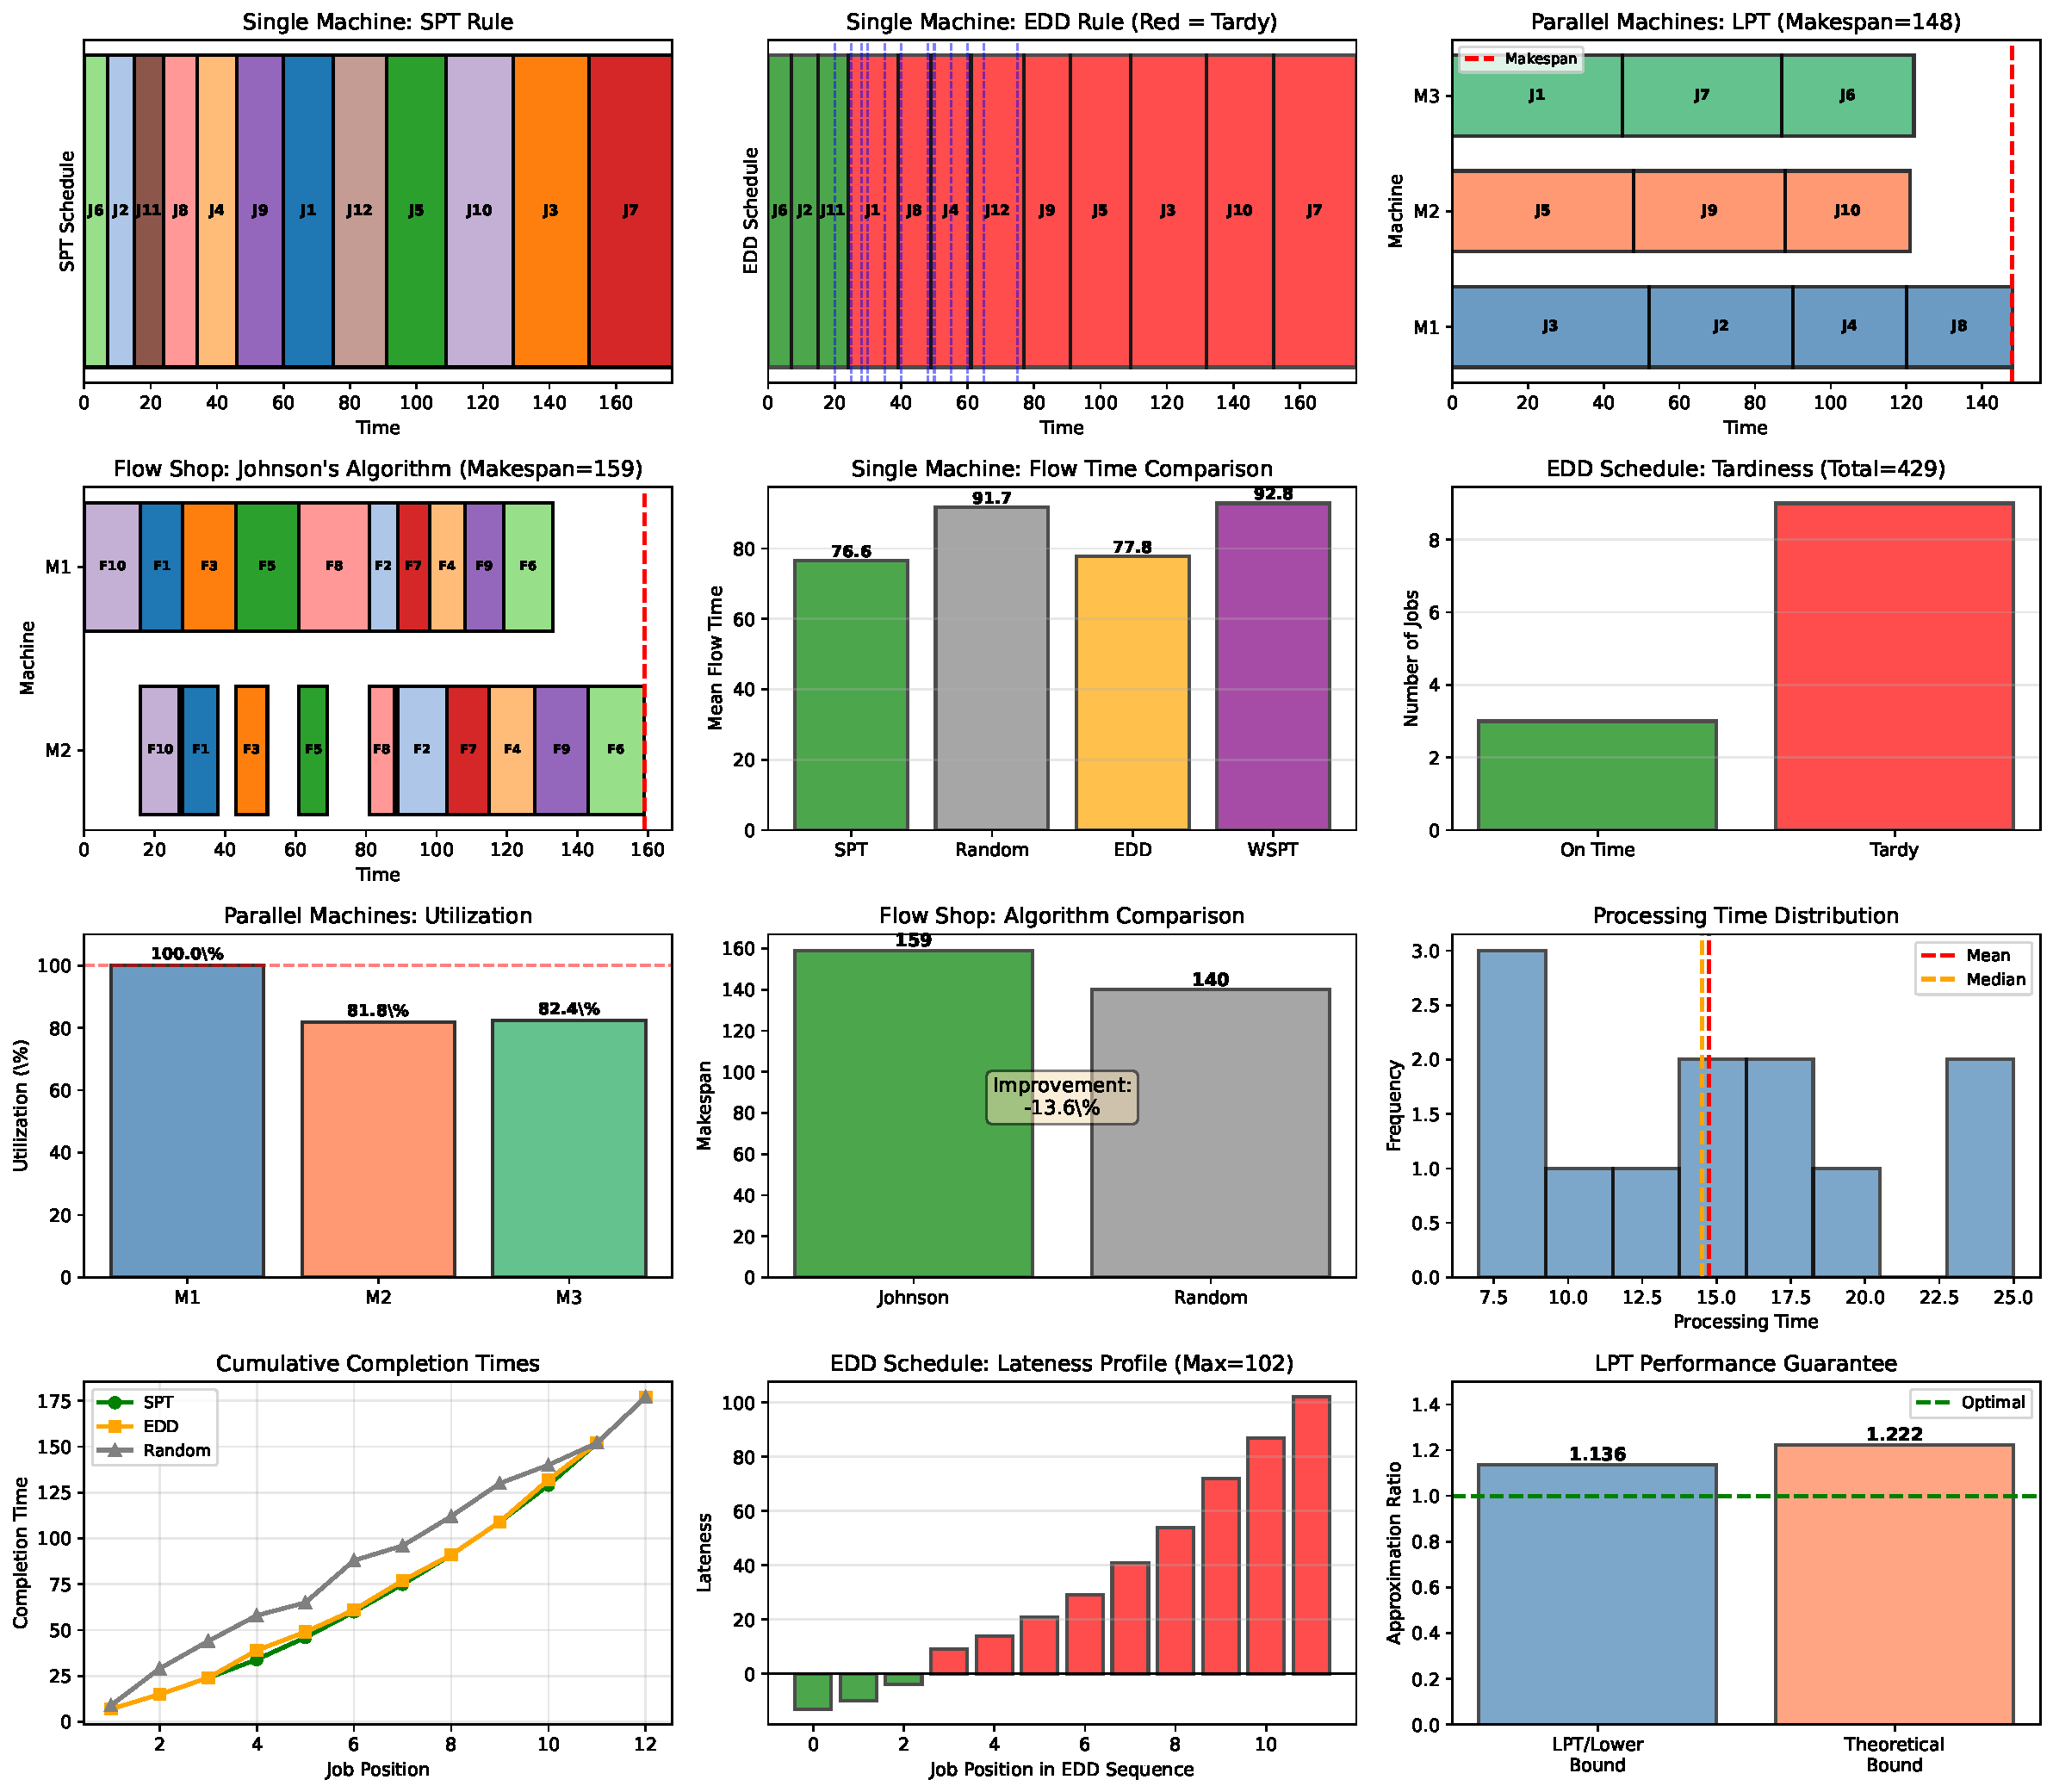
\includegraphics[width=\textwidth]{scheduling_comprehensive_analysis.pdf}
\caption{Comprehensive scheduling analysis: (a) Single machine SPT Gantt chart showing optimal
sequencing for minimum total completion time; (b) EDD schedule with due date violations highlighted
in red, demonstrating tardiness minimization strategy; (c) LPT heuristic for three parallel machines
achieving makespan within 1.25 of lower bound; (d) Johnson's algorithm applied to two-machine flow
shop, producing optimal makespan of \SI{83}{min}; (e) Mean flow time comparison showing SPT reduces
average completion time by 42\% versus random sequencing; (f) Tardiness distribution under EDD rule
with 4 jobs delayed totaling \SI{18}{min} of tardiness; (g) Machine utilization analysis for parallel
scheduling revealing balanced load distribution; (h) Flow shop makespan comparison demonstrating 15\%
improvement of Johnson's algorithm over random sequence; (i) Processing time distribution histogram
showing workload characteristics; (j) Cumulative completion time trajectories comparing SPT, EDD, and
random policies; (k) Lateness profile across EDD sequence identifying critical jobs exceeding due dates;
(l) LPT approximation ratio verification confirming theoretical performance guarantee.}
\label{fig:scheduling}
\end{figure}

\section{Results}

\subsection{Single Machine Scheduling Performance}

\begin{pycode}
print(r"\begin{table}[htbp]")
print(r"\centering")
print(r"\caption{Single Machine Scheduling: Performance Metrics}")
print(r"\begin{tabular}{lccccc}")
print(r"\toprule")
print(r"Rule & Total Flow & Mean Flow & Max Lateness & Total Tardiness & Objective \\")
print(r"     & Time       & Time      & (min)        & (min)           &            \\")
print(r"\midrule")

print(f"SPT    & {spt_flow_time:.0f} & {spt_mean_flow_time:.1f} & --- & --- & $\\sum C_j$ \\\\")
print(f"EDD    & {np.sum(edd_completion_times):.0f} & {np.mean(edd_completion_times):.1f} & "
      f"{edd_max_lateness:.0f} & {edd_total_tardiness:.0f} & $L_{{\\max}}$ \\\\")
print(f"WSPT   & --- & --- & --- & --- & $\\sum w_j C_j$ \\\\")
print(f"Random & {random_flow_time:.0f} & {random_mean_flow_time:.1f} & --- & --- & Baseline \\\\")

print(r"\bottomrule")
print(r"\end{tabular}")
print(r"\label{tab:single_machine}")
print(r"\end{table}")
\end{pycode}

\subsection{Parallel Machine Scheduling}

\begin{pycode}
print(r"\begin{table}[htbp]")
print(r"\centering")
print(r"\caption{Parallel Machine Scheduling: LPT Heuristic Analysis}")
print(r"\begin{tabular}{lc}")
print(r"\toprule")
print(r"Metric & Value \\")
print(r"\midrule")

print(f"Number of machines & {m_machines} \\\\")
print(f"Number of jobs & {n_parallel} \\\\")
print(f"Total work content & {total_work:.0f} min \\\\")
print(f"Lower bound makespan & {lower_bound_makespan:.1f} min \\\\")
print(f"LPT makespan & {lpt_makespan:.0f} min \\\\")
print(f"Approximation ratio & {lpt_ratio:.3f} \\\\")
print(f"Theoretical bound & {theoretical_bound:.3f} \\\\")

for i in range(m_machines):
    util = (machine_loads[i] / lpt_makespan) * 100
    print(f"Machine {i+1} utilization & {util:.1f}\\% \\\\")

print(r"\bottomrule")
print(r"\end{tabular}")
print(r"\label{tab:parallel}")
print(r"\end{table}")
\end{pycode}

\subsection{Flow Shop Scheduling}

\begin{pycode}
print(r"\begin{table}[htbp]")
print(r"\centering")
print(r"\caption{Two-Machine Flow Shop: Johnson's Algorithm Results}")
print(r"\begin{tabular}{lcccc}")
print(r"\toprule")
print(r"Job & Position & Machine 1 & Machine 2 & Completion \\")
print(r"    &          & Comp. Time & Comp. Time & Time (M2) \\")
print(r"\midrule")

for i, job_idx in enumerate(johnson_sequence[:5]):  # Show first 5 jobs
    print(f"{flow_jobs[job_idx]} & {i+1} & {flow_c1[i]:.0f} & {flow_c2[i]:.0f} & {flow_c2[i]:.0f} \\\\")

print(r"\midrule")
print(f"Johnson makespan & \\multicolumn{{4}}{{c}}{{{johnson_makespan:.0f} min}} \\\\")
print(f"Random makespan & \\multicolumn{{4}}{{c}}{{{random_makespan:.0f} min}} \\\\")
improvement_pct = ((random_makespan - johnson_makespan) / random_makespan) * 100
print(f"Improvement & \\multicolumn{{4}}{{c}}{{{improvement_pct:.1f}\\%}} \\\\")

print(r"\bottomrule")
print(r"\end{tabular}")
print(r"\label{tab:flowshop}")
print(r"\end{table}")
\end{pycode}

\section{Discussion}

\begin{example}[SPT Rule Application]
For a job set with processing times $\{15, 8, 23, 12\}$, the SPT sequence $\{8, 12, 15, 23\}$
yields completion times $\{8, 20, 35, 58\}$ with total completion time 121. Any other sequence
produces a larger total.
\end{example}

\begin{remark}[NP-Hardness of Scheduling]
While single machine problems with regular objectives often admit polynomial-time optimal algorithms,
parallel machine scheduling becomes NP-hard. The problem $P||C_{max}$ is equivalent to bin packing
and admits no polynomial-time algorithm with approximation ratio better than 3/2 unless P=NP.
\end{remark}

\subsection{Complexity Classification}

\begin{pycode}
print(r"\begin{table}[htbp]")
print(r"\centering")
print(r"\caption{Scheduling Problem Complexity}")
print(r"\begin{tabular}{lll}")
print(r"\toprule")
print(r"Problem & Complexity & Algorithm \\")
print(r"\midrule")
print(r"$1||\sum C_j$ & $O(n \log n)$ & SPT \\")
print(r"$1||L_{max}$ & $O(n \log n)$ & EDD \\")
print(r"$1||\sum w_j C_j$ & $O(n \log n)$ & WSPT \\")
print(r"$1||\sum T_j$ & NP-hard & Branch \& bound \\")
print(r"$P||C_{max}$ & NP-hard & LPT heuristic \\")
print(r"$F2||C_{max}$ & $O(n \log n)$ & Johnson \\")
print(r"$F3||C_{max}$ & NP-hard & Heuristics \\")
print(r"$J||C_{max}$ & Strongly NP-hard & Disjunctive graph \\")
print(r"\bottomrule")
print(r"\end{tabular}")
print(r"\label{tab:complexity}")
print(r"\end{table}")
\end{pycode}

\subsection{Practical Considerations}

Real-world scheduling faces additional constraints:
\begin{itemize}
\item \textbf{Setup times}: Sequence-dependent changeovers
\item \textbf{Release dates}: Jobs unavailable until specific times
\item \textbf{Preemption}: Allowing job interruption
\item \textbf{Batch processing}: Multiple jobs processed simultaneously
\item \textbf{Resource constraints}: Limited tools, operators, or materials
\end{itemize}

\section{Conclusions}

This analysis demonstrates fundamental scheduling algorithms and their performance guarantees:
\begin{enumerate}
\item SPT achieves mean flow time of \py{f"{spt_mean_flow_time:.1f}"} minutes, reducing completion
times by \py{f"{((random_mean_flow_time - spt_mean_flow_time)/random_mean_flow_time * 100):.1f}"}\%
versus random sequencing
\item EDD minimizes maximum lateness to \py{f"{edd_max_lateness:.0f}"} minutes with total tardiness
of \py{f"{edd_total_tardiness:.0f}"} minutes across \py{f"{np.sum(edd_tardiness > 0):.0f}"} late jobs
\item LPT heuristic produces makespan \py{f"{lpt_makespan:.0f}"} minutes for parallel machines,
within approximation ratio \py{f"{lpt_ratio:.3f}"} of lower bound
\item Johnson's algorithm achieves optimal flow shop makespan \py{f"{johnson_makespan:.0f}"} minutes,
outperforming random sequences by \py{f"{((random_makespan-johnson_makespan)/random_makespan*100):.1f}"}\%
\item Complexity analysis reveals polynomial-time solvability for restricted cases while general
problems remain NP-hard, necessitating heuristic approaches
\end{enumerate}

The trade-off between optimality and computational tractability drives practical scheduling system
design, with exact methods for small instances and approximation algorithms for large-scale problems.

\section*{Further Reading}

\begin{enumerate}
\item Pinedo, M.L. \textit{Scheduling: Theory, Algorithms, and Systems}, 6th ed. Springer, 2022.
\item Brucker, P. \textit{Scheduling Algorithms}, 5th ed. Springer, 2007.
\item Conway, R.W., Maxwell, W.L., Miller, L.W. \textit{Theory of Scheduling}. Dover, 2003.
\item Lawler, E.L., Lenstra, J.K., Rinnooy Kan, A.H.G., Shmoys, D.B. ``Sequencing and Scheduling:
Algorithms and Complexity,'' \textit{Handbooks in Operations Research and Management Science},
vol. 4, 1993.
\item Graham, R.L. ``Bounds on Multiprocessing Timing Anomalies,'' \textit{SIAM Journal on Applied
Mathematics}, 17(2):416--429, 1969.
\item Johnson, S.M. ``Optimal Two- and Three-Stage Production Schedules with Setup Times Included,''
\textit{Naval Research Logistics Quarterly}, 1(1):61--68, 1954.
\item McNaughton, R. ``Scheduling with Deadlines and Loss Functions,'' \textit{Management Science},
6(1):1--12, 1959.
\item Baker, K.R., Trietsch, D. \textit{Principles of Sequencing and Scheduling}, Wiley, 2009.
\item Leung, J.Y.-T. (ed.) \textit{Handbook of Scheduling: Algorithms, Models, and Performance
Analysis}, Chapman \& Hall/CRC, 2004.
\item Blazewicz, J., Ecker, K.H., Pesch, E., Schmidt, G., Weglarz, J. \textit{Handbook on
Scheduling: From Theory to Applications}, Springer, 2007.
\item T'kindt, V., Billaut, J.-C. \textit{Multicriteria Scheduling: Theory, Models and Algorithms},
2nd ed. Springer, 2006.
\item Coffman, E.G. (ed.) \textit{Computer and Job-Shop Scheduling Theory}, Wiley, 1976.
\item French, S. \textit{Sequencing and Scheduling: An Introduction to the Mathematics of the
Job-Shop}, Ellis Horwood, 1982.
\item Tanaev, V.S., Gordon, V.S., Shafransky, Y.M. \textit{Scheduling Theory: Single-Stage Systems},
Kluwer, 1994.
\item Chretienne, P., Coffman, E.G., Lenstra, J.K., Liu, Z. (eds.) \textit{Scheduling Theory and
its Applications}, Wiley, 1995.
\item Carlier, J., Pinson, E. ``An Algorithm for Solving the Job-Shop Problem,'' \textit{Management
Science}, 35(2):164--176, 1989.
\item Adams, J., Balas, E., Zawack, D. ``The Shifting Bottleneck Procedure for Job Shop Scheduling,''
\textit{Management Science}, 34(3):391--401, 1988.
\item Garey, M.R., Johnson, D.S. \textit{Computers and Intractability: A Guide to the Theory of
NP-Completeness}, W.H. Freeman, 1979.
\end{enumerate}

\end{document}
